\documentclass[a4paper,11pt]{article}

\usepackage[a4paper,margin=2.3cm]{geometry}
\usepackage{minted}
\usepackage{graphicx}
\usepackage{xcolor}
\usepackage{listings}

\definecolor{mGreen}{rgb}{0,0.6,0}
\definecolor{mGray}{rgb}{0.5,0.5,0.5}
\definecolor{mPurple}{rgb}{0.58,0,0.82}
\definecolor{backgroundColour}{rgb}{0.95,0.95,0.92}

\lstdefinestyle{CStyle}{
    backgroundcolor=\color{backgroundColour},   
    commentstyle=\color{mGreen},
    keywordstyle=\color{mBlue},
    numberstyle=\tiny\color{mRed},
    stringstyle=\color{mPurple},
    basicstyle=\footnotesize,
    breakatwhitespace=false,         
    breaklines=true,                 
    captionpos=b,                    
    keepspaces=true,                 
    numbers=left,                    
    numbersep=5pt,                  
    showspaces=false,                
    showstringspaces=false,
    showtabs=false,                  
    tabsize=2,
    language=C
}

\title{Layout of Heap Objects}
\author{Ruairidh MacGregor}
\date{}

\begin{document}

\maketitle

\section{Heap Objects}

All heap objects all contain a header, containing an \textbf{StgClosure}. A heap object always begins with a header, defined by \textbf{StgHeader}. Note: both structs are defined in "Closures.h".

\begin{lstlisting}[style=CStyle]
typedef struct {
    const struct StgInfoTable* info;
#ifdef PROFILING
    StgProfHeader         prof;
#endif
} StgHeader;
\end{lstlisting}

\begin{figure}[H]
    \centering
    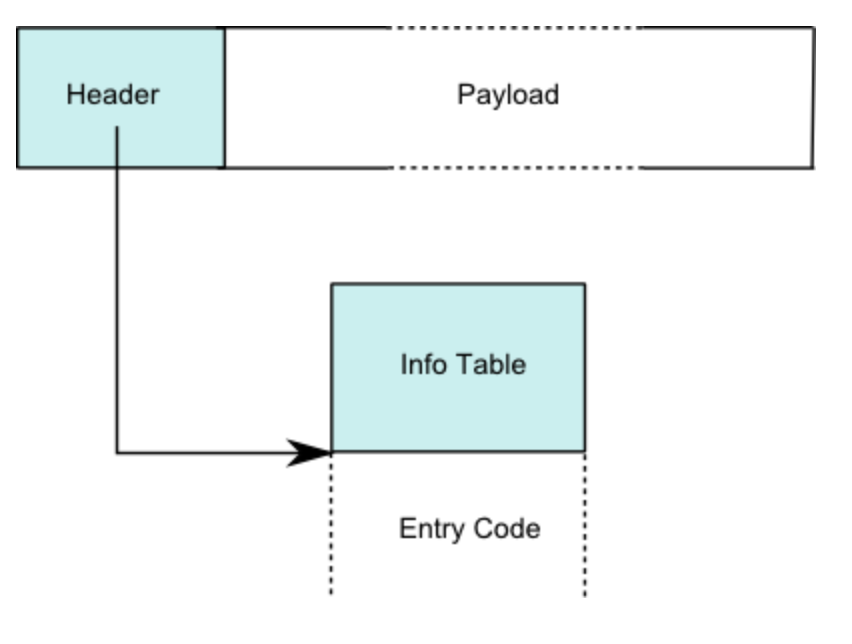
\includegraphics[width=\linewidth,height=0.7\linewidth]{GHC RTS Notes/Storage/images/header.png}
    \caption{The general layout for a closure. They all start with a StgHeader and then the payload.}
    \label{fig:header}
\end{figure}

The most important aspect of the \textbf{StgHeader} is the pointer to the StgInfoTable. This points to a table that contains information with regards to the closure.

\subsection{Info Tables}

The info table contains all the state required by the RTS about the closure. The struct is defined in "InfoTables.h".

\begin{figure}[H]
    \centering
    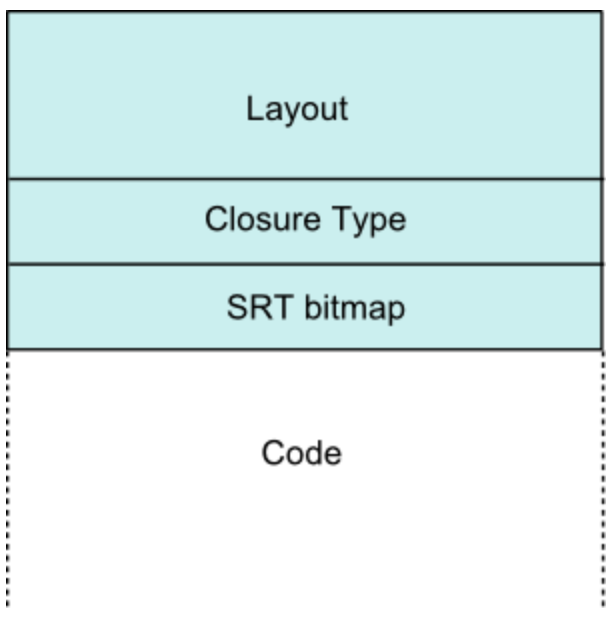
\includegraphics{GHC RTS Notes/Storage/images/infotable.png}
    \caption{}
    \label{fig:info_table}
\end{figure}

The \textbf{closure type} is a constant, defined in "ClosureTypes.h", it is simply a 16 bit unsigned integer. The \textbf{SRT bitmap} is used to support garbage collection of CAFs. The \textbf{layout} field describes the layout of the payload for the garbage collector. The \textbf{code} for the closure is usually the code that evaluates the closure.

\section{Payload Layout}

The GC needs to know 2 things about the payload of a heap object - how many words it contains and which of those words are pointers. There are 2 basic layouts for the payload: \textit{pointers-first} and \textit{bitmap}. It is a property of the closure type which determines this. Therefore, the GC checks the closure type to respond appropriately.

\subsection{Pointers-first Layout}

Payload consists of $\geq$ 0 pointers, followed by $\geq$ 0 non-pointers. Layout also contains two half-word-sized fields - number of (pointers|non-pointers)

\subsection{Bitmap Layout}

Payload consists of a mixture of pointers and non pointers, described by a bitmap.

The bitmap has layout: Bits 0-4 is the size of the payload and each bitmap entry in Bits 5-31 are 0 and 1, 0 iff the payload contains a pointer to a live object.

\section{Dynamic vs. Static Objects}

Objects fall into two categories:

\begin{description}
\item \textit{Dynamic} objects reside in the heap and may be moved by a garbage collector
\item \textit{Static} objects reside in compiled code, they are never moved because pointers are scattered throughout the object code and only the linker knows where
\end{description}

Useful MACRO: HEAP\_ALLOCED() from "rts/sm/HeapAlloc.h". Determine if an object is heap allocated or not.

\subsection{Dynamic Objects}

These have a minimum size, because every object must be big enough to be overwritten by a forwarding pointer. A forwarding pointer overwrites the original address of where the object was stored, to now point to the new location it has been moved to.

\subsection{Static Objects}

These have an additional field, called the static link field. The static link field is used by the GC to link all static objects, and so it can tell if it has visited a static object.

\section{Types of Objects}

\begin{description}
\item \textit{Data constructors}
\item \textit{Function closures}: a Haskell function
\item \textit{Thunks}: an unevaluted expression
\item \textit{Selector Thunks}: dynamically allocated thunk whose entry performs a simple selection operation, e.g. case <val> of
\item \textit{Partial Applications}: a function applied to too few arguments, e.g. x = map (\x -> x*2)
\item \textit{Generic Application}: applying a generic function to expressions
\item \textit{Stack Application}: computation of a thunk that was suspended halfway through
\item \textit{Indirections}: closures that point to other closures 
\item \textit{Byte Code Objects}: used in GHCi
\item \textit{Black Holes}: thunks that are being evaluated by another thread
\item \textit{Arrays}
\item \textit{MVars}
\item \textit{Weak pointers}: pointers that don't directly access an object, but can determine if it is still alive
\item \textit{Thread State Objects}: it represents the complete state of a thread
\item \textit{STM Objects}
\item \textit{Forwarding Pointers}: point to the new location an object has been moved to
\end{description}


\end{document}